\documentclass[10pt, aspectratio=169]{beamer}

% --- Theme Setup ---
\usetheme{Madrid}
\usecolortheme{default}
\setbeamercolor{palette primary}{bg=darkgray,fg=white}
\setbeamercolor{palette secondary}{bg=darkgray,fg=white}
\setbeamercolor{palette tertiary}{bg=darkgray,fg=white}
\setbeamercolor{structure}{fg=blue!70!black}

% --- Packages ---
\usepackage[utf8]{inputenc}
\usepackage[T1]{fontenc}
\usepackage{lmodern}
\usepackage{graphicx}
\usepackage{booktabs}
\usepackage{tikz}
\usetikzlibrary{shapes.geometric, arrows, positioning, calc, shadows, fit, backgrounds}
\usepackage{tabularx}

% --- TikZ Styles (Matching Report) ---
\tikzset{
    base/.style={text centered, font=\sffamily\small},
    startstop/.style={base, rectangle, rounded corners, minimum width=2.5cm, minimum height=0.8cm, draw=black, fill=blue!5, drop shadow, thick},
    io/.style={base, trapezium, trapezium left angle=70, trapezium right angle=110, minimum width=2cm, minimum height=0.8cm, draw=black, fill=blue!15, drop shadow, thick},
    process/.style={base, rectangle, minimum width=2.5cm, minimum height=0.8cm, draw=black, fill=orange!10, drop shadow, thick},
    decision/.style={base, diamond, aspect=1.5, minimum width=2.5cm, minimum height=0.8cm, draw=black, fill=green!10, drop shadow, thick},
    arrow/.style={thick,->,>=stealth, color=black},
    module/.style={rectangle, dashed, draw=black!50, fill=black!2, rounded corners, inner sep=10pt}
}

% --- Metadata ---
\title[Video Summarization]{Dynamic Video Summarization via Bidirectional RNNs and Transformer Architectures}
\subtitle{Course Project: Deep Learning (DSAI 308)}
\author[Yasser, Hazem, Ashraf]{Amr Yasser, Omar Hazem, Ali Ashraf}
\institute[DSAI]{
    Deep Learning \\
    Supervisor: \textbf{Dr. Khaled El-Sayed}
}
\date{Fall 2025}

% --- Slides ---
\begin{document}

% 1. Title Slide
\begin{frame}
    \titlepage
\end{frame}

% 2. Table of Contents
\begin{frame}{Outline}
    \tableofcontents
\end{frame}

\section{Introduction}

% 3. Motivation
\begin{frame}{Motivation \& Problem Definition}
    \begin{itemize}
        \item \textbf{Explosion of Video Content:} Massive growth in platforms requires automated navigation.
        \item \textbf{Video Summarization:} Generating a concise, representative summary (static keyframes).
        \item \textbf{Challenges:}
        \begin{itemize}
            \item Capturing long-range temporal dependencies.
            \item Balancing redundancy vs. information salience.
            \item Handling diverse video domains (narratives vs. action).
        \end{itemize}
    \end{itemize}
    \vfill
    \begin{figure}
        \centering
        \includegraphics[width=0.4\textwidth]{../results/figures/4wU_LUjG5Ic_qualitative.png}
        \caption{\small Sample detection for TVSum category "Parade".}
    \end{figure}
\end{frame}

\section{Methodology}

% 4. Pipeline
\begin{frame}{System Architecture: Two-Stage Pipeline}
    \centering
    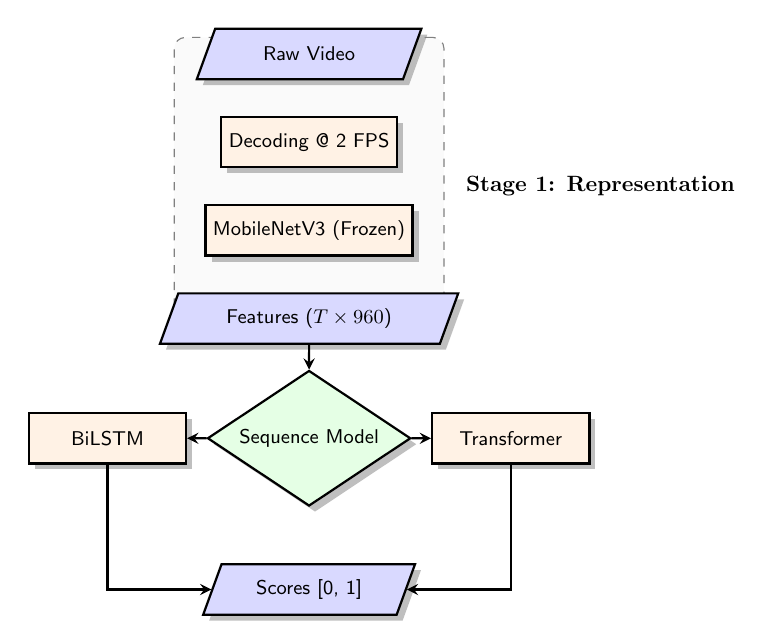
\begin{tikzpicture}[node distance=1.4cm, auto, scale=0.8, every node/.style={scale=0.8}]
        % Stage 1
        \node (in) [io] {Raw Video};
        \node (proc) [process, below of=in] {Decoding @ 2 FPS};
        \node (cnn) [process, below of=proc] {MobileNetV3 (Frozen)};
        \node (feat) [io, below of=cnn] {Features ($T \times 960$)};
        
        \begin{scope}[on background layer]
            \node [module, fit=(in) (feat)] (s1) {};
            \node at (s1.east) [right=5pt, font=\bfseries] {Stage 1: Representation};
        \end{scope}

        % Stage 2
        \node (model) [decision, below of=feat, yshift=-0.5cm] {Sequence Model};
        \node (bilstm) [process, left of=model, xshift=-1.8cm] {BiLSTM};
        \node (trans) [process, right of=model, xshift=1.8cm] {Transformer};
        \node (score) [io, below of=model, yshift=-1cm] {Scores [0, 1]};

        \draw [arrow] (feat) -- (model);
        \draw [arrow] (model) -- (bilstm);
        \draw [arrow] (model) -- (trans);
        \draw [arrow] (bilstm) |- (score);
        \draw [arrow] (trans) |- (score);
    \end{tikzpicture}
\end{frame}

\section{Deep Sequence Modeling}

% 5. BiLSTM
\begin{frame}{BiLSTM: Sequential Contextualization}
    \begin{columns}
        \column{0.5\textwidth}
        \begin{block}{Architecture}
            \begin{itemize}
                \item 512-dim Bottleneck Projection.
                \item 2-layer Bidirectional LSTM.
                \item MLP Regression Head.
            \end{itemize}
        \end{block}
        \begin{block}{Intuition}
            \begin{itemize}
                \item Models local flow (past/future dependencies).
                \item Superior for narrative continuity.
            \end{itemize}
        \end{block}
        
        \column{0.5\textwidth}
        \centering
        \[ h_t = [ \overrightarrow{f}(x_t, h_{t-1}) ; \overleftarrow{b}(x_t, h_{t+1}) ] \]
        \vfill
        \includegraphics[width=0.8\textwidth]{../results/figures/Bhxk-O1Y7Ho_qualitative.png}
    \end{columns}
\end{frame}

% 6. Transformer
\begin{frame}{Transformer: Global Dependencies}
    \begin{columns}
        \column{0.5\textwidth}
        \begin{block}{Architecture}
            \begin{itemize}
                \item Sinusoidal Positional Encoding.
                \item 4-Head Self-Attention.
                \item Dense Head for Score Regression.
            \end{itemize}
        \end{block}
        \begin{block}{Intuition}
            \begin{itemize}
                \item Non-local relationship modeling.
                \item Correctly identifies sparse climax events.
            \end{itemize}
        \end{block}

        \column{0.5\textwidth}
        \centering
        \[ \text{Attn}(Q, K, V) = \text{softmax}\left( \frac{QK^T}{\sqrt{d_k}} \right)V \]
        \vfill
        \includegraphics[width=0.8\textwidth]{../results/figures/JgHubY5Vw3Y_qualitative.png}
    \end{columns}
\end{frame}

\section{Results \& Analysis}

% 7. Quantitative Results
\begin{frame}{Quantitative Evaluation (TVSum)}
    \begin{table}
        \centering
        \caption{Supervised Results on TVSum}
        \begin{tabular}{lcccc}
            \toprule
            \textbf{Model} & \textbf{Spearman $\rho$} & \textbf{Kendall $\tau$} & \textbf{MSE} & \textbf{MAE} \\ \midrule
            \textbf{BiLSTM} & \textbf{0.531} & \textbf{0.362} & 0.0142 & 0.092 \\
            \textbf{Transformer} & 0.418 & 0.285 & 0.0191 & 0.104 \\ \bottomrule
        \end{tabular}
    \end{table}
    \begin{itemize}
        \item \textbf{Key Finding:} BiLSTM excels at sequential tasks (tutorial, vlogs).
        \item \textbf{Observation:} Transformer shows higher robustness in non-linear action sequences.
    \end{itemize}
\end{frame}

% 8. Transfer Learning
\begin{frame}{Transfer Learning on SumMe Dataset}
    \centering
    \includegraphics[width=0.8\textwidth]{../results/figures/summe_fscore_sorted.png}
    \vfill
    \begin{itemize}
        \item Successful zero-shot transfer from TVSum $\rightarrow$ SumMe.
        \item Models successfully identify climax moments even in unseen domains.
    \end{itemize}
\end{frame}

% 9. Qualitative Comparison: Cars Video
\begin{frame}{Qualitative Comparison: Cars Demo Video}
    \begin{columns}
        \column{0.5\textwidth}
        \centering
        \textbf{BiLSTM Selection}
        \vfill
        \includegraphics[width=0.45\textwidth]{../results/demo_outputs/cars/keyframes/bilstm/kf_0018.jpg}
        \includegraphics[width=0.45\textwidth]{../results/demo_outputs/cars/keyframes/bilstm/kf_0066.jpg}
        \vfill
        \includegraphics[width=0.45\textwidth]{../results/demo_outputs/cars/keyframes/bilstm/kf_0103.jpg}
        
        \column{0.5\textwidth}
        \centering
        \textbf{Transformer Selection}
        \vfill
        \includegraphics[width=0.45\textwidth]{../results/demo_outputs/cars/keyframes/transformer/kf_0073.jpg}
        \includegraphics[width=0.45\textwidth]{../results/demo_outputs/cars/keyframes/transformer/kf_0084.jpg}
        \vfill
        \includegraphics[width=0.45\textwidth]{../results/demo_outputs/cars/keyframes/transformer/kf_0105.jpg}
    \end{columns}
    \vfill
    \begin{itemize}
        \item \textbf{BiLSTM:} More uniform coverage of the sequence.
        \item \textbf{Transformer:} Identical focus on climax frames (car entry).
    \end{itemize}
\end{frame}

% 10. Qualitative Comparison: AI Robot
\begin{frame}{Qualitative Comparison: AI Robot Demo Video}
    \begin{columns}
        \column{0.5\textwidth}
        \centering
        \textbf{BiLSTM Selection}
        \vfill
        \includegraphics[width=0.45\textwidth]{../results/demo_outputs/ai_robot/keyframes/bilstm/kf_0004.jpg}
        \includegraphics[width=0.45\textwidth]{../results/demo_outputs/ai_robot/keyframes/bilstm/kf_0007.jpg}
        
        \column{0.5\textwidth}
        \centering
        \textbf{Transformer Selection}
        \vfill
        \includegraphics[width=0.45\textwidth]{../results/demo_outputs/ai_robot/keyframes/transformer/kf_0002.jpg}
        \includegraphics[width=0.45\textwidth]{../results/demo_outputs/ai_robot/keyframes/transformer/kf_0009.jpg}
    \end{columns}
    \vfill
    \begin{itemize}
        \item \textbf{Comparison:} Models agree on high-importance action frames.
        \item \textbf{Budget:} 15\% frame budget maintained per selection logic.
    \end{itemize}
\end{frame}

\section{Conclusion}

% 9. Conclusion
\begin{frame}{Conclusion \& Future Work}
    \begin{block}{Summary}
        \begin{itemize}
            \item Built an E2E pipeline: decoding, features, modeling, selection.
            \item BiLSTM is the reliable choice for steady temporal flows.
            \item Transformers offer better global reasoning for sparse highlights.
        \end{itemize}
    \end{block}
    \vfill
    \begin{block}{Future Directions}
        \begin{itemize}
            \item \textbf{Multimodal Fusion:} Integrating Audio/Text signals.
            \item \textbf{Unsupervised Learning:} Scaling with SUM-GAN/Contrastive learning.
        \end{itemize}
    \end{block}
\end{frame}

% 10. Q&A
\begin{frame}
    \centering
    \Huge \textbf{Questions?}
    \vfill
    \Large \textit{Thank You!}
\end{frame}

\end{document}
